\documentclass[letterpaper,10pt]{article}
\usepackage[margin=2cm]{geometry}

\usepackage{graphicx}
\usepackage{amsmath}
\usepackage{amsfonts}
\usepackage{amssymb}
\usepackage[colorlinks]{hyperref}

\DeclareMathOperator*{\argmin}{arg\,min}
\DeclareMathOperator*{\argmax}{arg\,max}

\newcommand{\pandochline}{\vspace{2em}\href{./document.html}{\textbf{Back to Top}}
	\vspace{-2em}\begin{center}\rule{\textwidth}{1pt}\end{center}}

\setlength{\parindent}{0em}
\setlength{\parskip}{1em}

\title{\textbf{18794 Pattern Recognition Theory\\Prof. Marios Savvides}}
\author{HMW-Alexander}

\begin{document}
	
\maketitle

\tableofcontents
\newpage

\section{Introduction}

\pandochline
\section{Decision Theory}

\subsection{Terms}

\begin{itemize}
	\item Feature Space:
	\begin{itemize}
		\item \textbf{Feature}: a distinctive characteristic or quality of the object
		\item \textbf{Feature vector}: combine more than one feature as a vector
		\item \textbf{Feature space}: The space defined by the feature vectors
	\end{itemize}
	\item Classifiers:
	\begin{itemize}
		\item \textbf{Decision regions}: a classifier partitions the feature space into class-corresponding decision regions.
		\item \textbf{Decision boundaries}: the borders between the decision regions.
	\end{itemize}
\end{itemize}

\subsection{Bayes Rule}

\begin{equation}
P(w_i|x)=\frac{P(x,w_i)}{P(x)}=\frac{P(x|w_i)P(w_i)}{\sum_{k=1}^{C}{P(x|w_k)P(w_k)}}
\end{equation}
\begin{itemize}
	\item \textbf{Posterior Probability} $P(w_i|x)$: the conditional probability of correct class being $w_i$ given that feature value $x$ has been observed.
	\item \textbf{Evidence} $P(x)$: the total probability of observing the feature value of $x$.
	\item \textbf{Likelihood} $P(x|w_i)$: the conditional probability of observing a feature value of $x$ given that the correct class is $w_i$.
	\item \textbf{Prior Probability} $P(w_i)$: the probability of class $w_i$, $\sum_{k=1}^{C}{P(w_k)}=1$.
	\item \textbf{Bayes Classifiers} decide on the class that has the \textbf{largest posterior probability} ($\max_{w_i}{P(w_i|x)}$). They are statistically the best classifiers i.e. they are minimum error classifiers (optimal).
\end{itemize}

\subsection{Minimum Probability of Error}

\begin{itemize}
	\item $\epsilon=P(error|class)$: probability of assigning $x$ to the wrong class $w$.
	\item $P_e=\sum_{k=1}^{C}{P(w_k)\epsilon_k}$: total probability of error.
\end{itemize}
\begin{figure}[!ht]
	\centering
	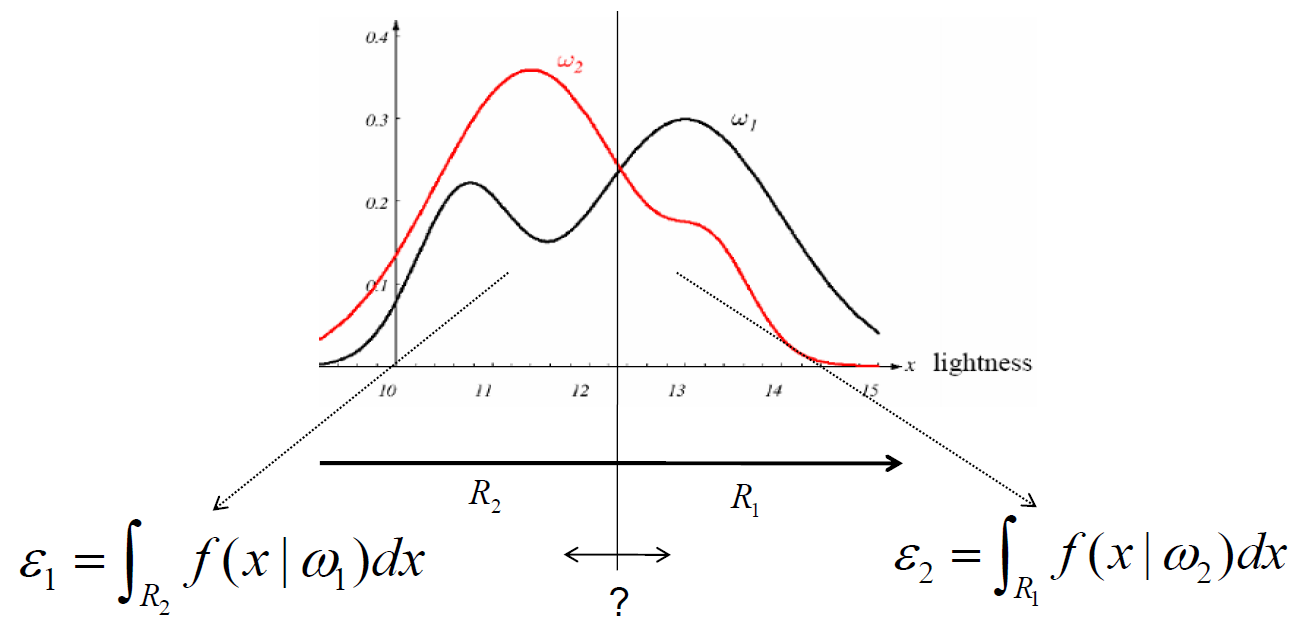
\includegraphics[width=10cm]{./img/minimum_probability_of_error.png}
\end{figure}
For the two class case shown above, we want to minimize $P_e$ as below:
\begin{equation}
\begin{array}{rcl}
P_e & = & P(w_1)\epsilon_1 + P(w_2)\epsilon_2 \\
	& = & P(w_1)\int_{R_2}{f(x|w_1)dx} + P(w_2)\int_{R_1}{f(x|w_2)dx} \\
	& = & P(w_1)(1-\int_{R_1}{f(x|w_1)dx}) + P(w_2)\int_{R_1}{f(x|w_2)dx} \\
	& = & P(w_1) + \int_{R_1}{(P(w_2)f(x|w_2) - P(w_1)f(x|w_1))dx} \\ 
\end{array}
\end{equation}
To minimize $P_e$, we want $P(w_2)f(x|w_2) - P(w_1)f(x|w_1)$ to be always negative$(<0)$ in the region $R_1$:
\begin{equation}
\begin{array}{rcl}
P(w_1)f(x|w_1) - P(w_2)f(x|w_2) >0 & \Rightarrow & w_1 \\
P(w_1)f(x|w_1) - P(w_2)f(x|w_2) <0 & \Rightarrow & w_2 \\
\end{array}
\end{equation}

\subsection{Likelihood Ratio}

\begin{itemize}
	\item \textbf{Likelihood ratio}: $l(x)=\frac{f(x|w_1)}{f(x|w_2)}$
	\item \textbf{Log likelihood ratio}: $\ln(l(x))=\ln(\frac{f(x|w_1)}{f(x|w_2)})=\ln(f(x|w_1))-\ln(f(x|w_2))$
	\item \textbf{Ratio of a priori probabilities}: $T=\frac{P(w_2)}{P(w_1)}$
	\item \textbf{Log ratio of a priori probabilities}: $\ln(T)=\ln(\frac{P(w_2)}{P(w_1)})=\ln(P(w_2))-\ln(P(w_1))$
\end{itemize}

\begin{equation}
\begin{array}{rcl}
\ln(l(x)) = \ln(\frac{f(x|w_1)}{f(x|w_2)}) > \ln(\frac{P(w_2)}{P(w_1)}) = \ln(T) & \Rightarrow & w_1 \\
\ln(l(x)) = \ln(\frac{f(x|w_1)}{f(x|w_2)}) < \ln(\frac{P(w_2)}{P(w_1)}) = \ln(T) & \Rightarrow & w_2 \\
\end{array}
\end{equation}

\subsubsection{Likelihood as Gaussian distribution}
Assume likelihood $f(x|w_i)$ are Gaussian distributions with mean $\mu_i$ and variance $\sigma_i^2$.
\begin{equation}
f(x|w_i)=\frac{1}{\sqrt{2\pi\sigma_i^2}}\exp\left(-\frac{(x-\mu_i)^2}{2\sigma_i^2}\right)
\end{equation}
\begin{figure}[!ht]
	\centering
	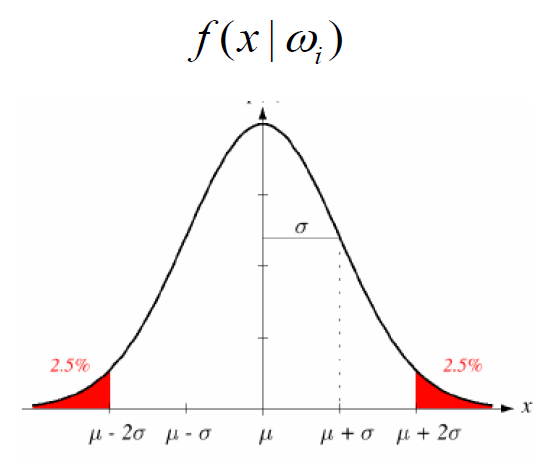
\includegraphics[width=6cm]{./img/gaussian_distribution_likelihood.png}
\end{figure}
The log likelihood ratio:
\begin{equation}
\begin{array}{rcl}
\ln(l(x)) & = & \ln\left(\frac{\frac{1}{\sqrt{2\pi\sigma_1^2}}\exp\left(-\frac{(x-\mu_1)^2}{2\sigma_1^2}\right)}{\frac{1}{\sqrt{2\pi\sigma_2^2}}\exp\left(-\frac{(x-\mu_2)^2}{2\sigma_2^2}\right)}\right) \\
         & = & \ln(\frac{\sigma_2}{\sigma_1})+\frac{(x-\mu_2)^2}{2\sigma_2^2}-\frac{(x-\mu_1)^2}{2\sigma_1^2}
\end{array}
\end{equation}

Case: $\sigma_1=\sigma_2=\sigma$
\begin{equation}
\begin{array}{rcl}
\ln(l(x)) & = & \frac{2x(\mu_1-\mu_2)-(\mu_1^2-\mu_2^2)}{2\sigma^2}
\end{array}
\end{equation}

\begin{equation}
\begin{array}{rcl}
x(\mu_1-\mu_2) - \frac{\mu_1^2-\mu_2^2}{2} > \sigma^2 \ln(\frac{P(w_2)}{P(w_1)}) & \Rightarrow & w_1 \\
x(\mu_1-\mu_2) - \frac{\mu_1^2-\mu_2^2}{2} < \sigma^2 \ln(\frac{P(w_2)}{P(w_1)}) & \Rightarrow & w_2 \\
\end{array}
\end{equation}

If $P(w_1)=P(w_2)$
\begin{equation}
x = \frac{\mu_1+\mu_2}{2}
\end{equation}

\begin{figure}[!ht]
	\centering
	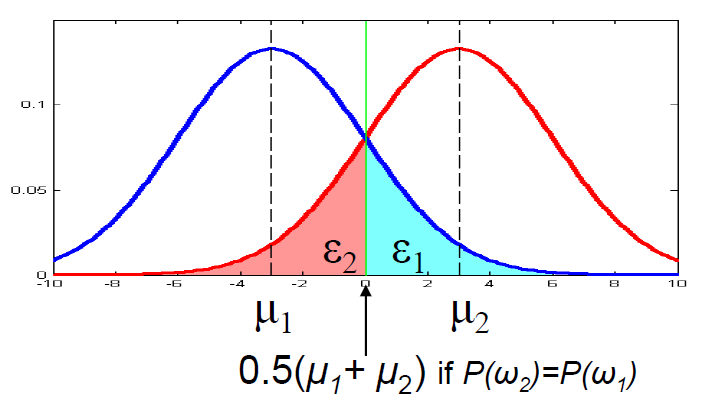
\includegraphics[width=8cm]{./img/gaussian_linear_classifier.png}
\end{figure}

Case: $\sigma_1\neq\sigma_2$

\begin{figure}[!ht]
	\centering
	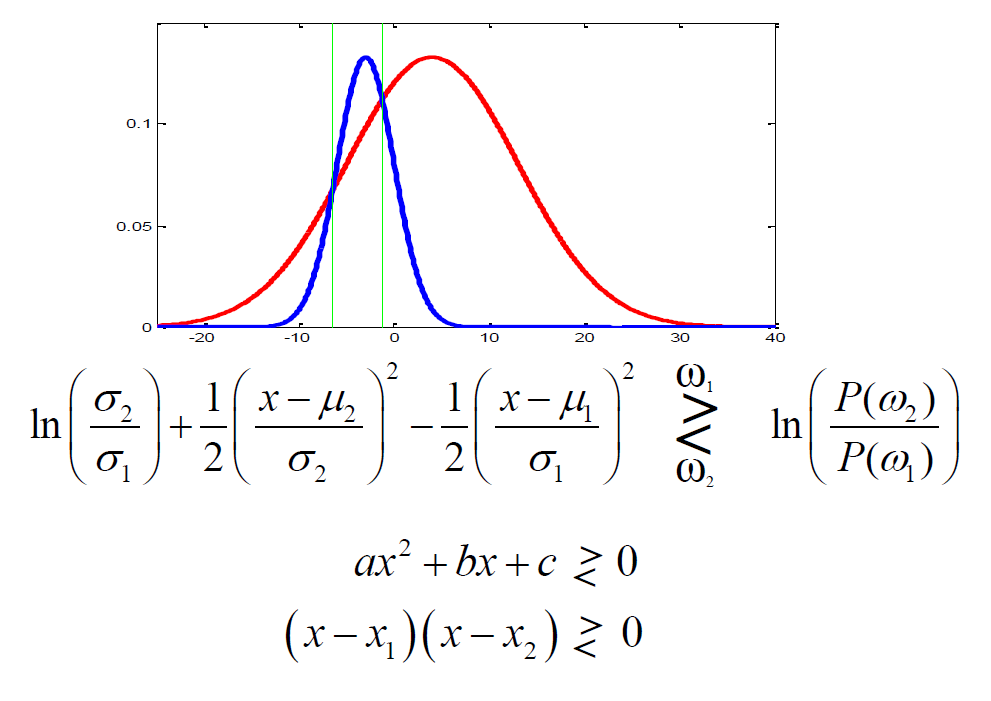
\includegraphics[width=8cm]{./img/guassian_quadratic_classifier.png}
\end{figure}

\pandochline
\section{Parametric \& Non-Parametric Density Estimation}

Learning \& Classification
\begin{itemize}
	\item Supervised:
	\begin{itemize}
		\item Bayes Density:
		\begin{itemize}
			\item Parametric: assumes a particular form of a PDF (e.g. Gaussian) is known $\rightarrow$ determine the parameters (e.g. mean and variance)
			\begin{itemize}
				\item Maximum Likelihood ($f(x|w_i)$) Estimation (MLE)
				\item Maximum A Posteriori (Bayesian $p(w_i|x)$) Estimation (MAPE)
			\end{itemize}
			\item Non-Parametric: no assumption about the density
			\begin{itemize}
				\item Parzen Windows
				\item Kernel Density Estimation
				\item K-Nearest Neighbor Rule
			\end{itemize}
		\end{itemize}
		\item Discriminant Analysis:
		\begin{itemize}
			\item Linear
			\item Non-Linear
		\end{itemize}
	\end{itemize}
	\item Unsupervised:
	\begin{itemize}
		\item Clustering
	\end{itemize}
\end{itemize}

\subsection{ML Estimation (MLE)}
Steps:
\begin{itemize}
	\item Assume $P(x|w)$ has a known parametric form uniquely determined by the parameter vector $\theta$
	\item The parameters are assumed to be fixed (i.e. non random) but unknown
	\item Suppose we have a dataset $D$ with the samples in $D$ having been drawn \textbf{independently} according to the probability law $P(x|w)$
	\item The MLE is the value of $\theta$ that best explains the data and once we know this value, we know $P(x|w)$
	\begin{equation}
	\hat{\theta}=\argmax_\theta\{P(D|\theta)\}=\argmax_\theta\{\prod_{k=1}^{N}{P(x_k|\theta)}\}=\argmax_\theta\{\sum_{k=1}^{N}{\log(P(x_k|\theta))}\}
	\end{equation}
	Choose the value of $\theta$ that is the most likely to give rise to the data we observe.
\end{itemize}

Method:
\begin{itemize}
	\item Assume $\theta=[\theta_1,\theta_2,\dots,\theta_p]^T$
	\item Assume gradient operator $\nabla_\theta=[\frac{\partial}{\partial\theta_1},\frac{\partial}{\partial\theta_2},\dots,\frac{\partial}{\partial\theta_p}]^T$
	\item Assume the log-likelihood of the objective function $l(\theta)=\sum_{k=1}^{N}{\log(P(x_k|\theta))}$
	\item Therefore: $\nabla_\theta l(\theta)=\sum_{k=1}^{N}{\nabla_\theta \log(P(x_k|\theta))}=0$
\end{itemize}

\subsubsection{E.g. Univariate Gaussian}

\begin{equation}
P(x|\mu,\sigma^2)=\frac{1}{\sqrt{2\pi\sigma^2}}\exp(-\frac{(x-\mu)^2}{2\sigma^2})
\end{equation}

\begin{equation}
\theta=\left[\begin{array}{c}
\theta_1=\mu \\
\theta_2=\sigma^2 \\
\end{array}\right]
\end{equation}

\begin{equation}
\begin{array}{rcl}
\log(P(x_k|\theta)) & = & \log(\frac{1}{\sqrt{2\pi\theta_2}}\exp(-\frac{(x_k-\theta_1)^2}{2\theta_2})) \\
                   & = & -\frac{1}{2}\log(2\pi\theta_2)-\frac{(x_k-\theta_1)^2}{2\theta_2} \\
\end{array}
\end{equation}

\begin{equation}
\begin{array}{rcl}

\nabla_\theta \log(P(x_k|\theta)) & = & \left[
\begin{array}{c}
\frac{x_k-\theta_1}{\theta_2} \\
-\frac{1}{2\theta_2}+\frac{(x_k-\theta_1)^2}{2\theta_2} \\
\end{array}\right] \\

\Rightarrow \left\{
\begin{array}{rcl}
\sum_{k=1}^{n}{\frac{1}{\theta_2}(x_k-\theta_1)} & = & 0 \\
-\sum_{k=1}^{n}{\frac{1}{\theta_2}}+\sum_{k=1}^{n}{\frac{(x_k-\theta_1)^2}{\theta_2^2}} & = & 0 \\
\end{array}\right. & \Rightarrow & \left\{
\begin{array}{rcl}
\hat{\mu} & = & \frac{1}{n}\sum_{k=1}^{n}{x_k} \\
\hat{\sigma}^2 & = & \frac{1}{n}\sum_{k=1}^{n}{(x_k-\hat{\mu})^2} \\
\end{array}\right. \\

\end{array}
\end{equation}

\subsubsection{E.g. Multivariate Gaussian}

\begin{equation}
P(x|\mu,\Sigma)=\frac{1}{(2\pi)^{d/2}|\Sigma|^{1/2}}\exp(-\frac{1}{2}(x-\mu)^T\Sigma^{-1}(x-\mu))
\end{equation}

Case: only the mean $\mu$ is unknown

\begin{equation}
\log(P(x_k|\mu)) = -\frac{1}{2}\log((2\pi)^{d}|\Sigma|)-\frac{1}{2}(x_k-\mu)^T\Sigma^{-1}(x_k-\mu)
\end{equation}

\begin{equation}
\begin{array}{rcl}
\nabla_\theta \log(P(x_k|\mu)) & = & \Sigma^{-1}(x_k-\mu) \\
\Rightarrow \sum_{k=1}^{n}{\Sigma^{-1}(x_k-\mu)} = 0 & \Rightarrow & \hat{\mu} = \frac{1}{n}\sum_{k=1}^{n}{x_k}
\end{array}
\end{equation}

Case: Neither the mean $\mu$ nor the covariance matrix $\Sigma$ are known

\begin{equation}
\theta=\left[\begin{array}{rcl}
\theta_1 & = & \mu \\
\theta_2 & = & \Sigma \\
\end{array}\right]
\end{equation}

Convert the covariance matrix $\Sigma$

\begin{equation}
\begin{array}{rcl}
P(D|\Sigma) & = & \prod_{k=1}^{n}{P(x_k|\Sigma)} \\
			& = & \prod_{k=1}^{n}{\frac{1}{\sqrt{(2\pi)^d|\Sigma|}}\exp(-\frac{1}{2}(x_k-\mu)^T\Sigma^{-1}(x_k-\mu))} \\
			& = & \frac{1}{((2\pi)^d|\Sigma|)^{n/2}}\exp(-\frac{1}{2}\sum_{n}^{k=1}{(x_k-\mu)^T\Sigma^{-1}(x_k-\mu)}) \\
\end{array}
\end{equation}

The property of matrix trace 
\begin{itemize}
	\item scalar $b^TBb=trace(b^TBb)=trace(Bbb^T)$
	\item $trace(A+B)=trace(A)+trace(B)$
	\item $trace(C(A+B))=trace(CA)+trace(CB)$
	\item $trace(A)$ is the sum of $A$'s eigenvalues
\end{itemize}

\begin{equation}
\begin{array}{rcl}
\sum_{n}^{k=1}{(x_k-\mu)^T\Sigma^{-1}(x_k-\mu)} & = & \sum_{n}^{k=1}{trace((x_k-\mu)^T\Sigma^{-1}(x_k-\mu))} \\
												& = & \sum_{n}^{k=1}{trace(\Sigma^{-1}(x_k-\mu)(x_k-\mu)^T)} \\
												& = & trace(\Sigma^{-1}\sum_{n}^{k=1}{(x_k-\mu)(x_k-\mu)^T})\\												
\end{array}
\end{equation}

Assume
\begin{equation}
A=\frac{1}{n}\sum_{k=1}^{n}(x_k-\mu)(x_k-\mu)^T
\end{equation}
and $A$ is fixed.

Then
\begin{equation}
\sum_{n}^{k=1}{(x_k-\mu)^T\Sigma^{-1}(x_k-\mu)} = n~trace(\Sigma^{-1}A)
\end{equation}

Therefore
\begin{equation}
P(D|\Sigma) = \frac{1}{((2\pi)^d|\Sigma|)^{n/2}}\exp(-\frac{n}{2}trace(\Sigma^{-1}A))
\end{equation}

Assume
\begin{equation}
B=\Sigma^{-1}A
\end{equation}
and B's eigenvalues are $\lambda_1,\lambda_2,\dots,\lambda_d$

The property of matrix determinant
\begin{itemize}
	\item $det(AB)=det(A)det(B)$
	\item $det(A^{-1})=det(A)^{-1}$
	\item $det(A)$ is the product of $A$'s eigenvalues
\end{itemize}

Therefore
\begin{equation}
\begin{array}{rcl}
P(D|\Sigma) & = & \frac{1}{((2\pi)^d|\Sigma|)^{n/2}}\exp(-\frac{n}{2}trace(\Sigma^{-1}A)) \\
			& = & \frac{1}{(2\pi)^{dn/2}}|\Sigma|^{-n/2}\exp(-\frac{n}{2}trace(B)) \\
			& = & \frac{1}{(2\pi)^{dn/2}}(\frac{|B|}{|A|})^{n/2}\exp(-\frac{n}{2}trace(B)) \\
			& = & \frac{1}{(2\pi)^{dn/2}}|A|^{-n/2}(\prod_{i=1}^{d}{\lambda_i})^{n/2}\exp(-\frac{n}{2}\sum_{i=1}^{d}{\lambda_i}) \\
\end{array}
\end{equation}

\begin{equation}
\log(P(D|\Sigma))=-\frac{dn}{2}\log(2\pi)-\frac{n}{2}\log(|A|)+\frac{n}{2}\sum_{i=1}^{d}{\log(\lambda_i)}-\frac{n}{2}\sum_{i=1}^{d}{\lambda_i}
\end{equation}

\begin{equation}
\frac{\partial(\log(P(x|\Sigma)))}{\partial\lambda_i}=\frac{n}{2\lambda_i}-\frac{n}{2}=0 \Rightarrow \lambda_i=1
\end{equation}

Therefore $B \sim I$, and $\Sigma^{-1}A=I \Rightarrow \hat{\Sigma}=A=\frac{1}{n}\sum_{k=1}^{n}(x_k-\mu)(x_k-\mu)^T$.

\subsection{Bayesian Estimation (BE)}
Steps:
\begin{itemize}
	\item The parameters are assumed to be random variables with some known priori distribution.
	\item Bayesian approach aims at estimating the posterior density $P(\theta|D)$
	\item The MAPE(Maximum A Posteriori Estimate) of $\theta$ is the value of $\theta$ that maximizes the posterior density $P(\theta|D)$.
\end{itemize}
Method:
\begin{itemize}
	\item Estimate $P(x|D)$ from sample data, and assume it has a known parametric form. So $P(x|\theta)$ is completely known, but $\theta$ is random variable and has its own PDF.
	\item $P(x|D)=\int{P(x,\theta|D)d\theta}=\int{P(x|\theta)P(\theta|D)d\theta}$
	\item Posterior $P(\theta|D)=\frac{P(D|\theta)P(\theta)}{P(D)}$, where $P(D|\theta)=\prod_{k=1}^{n}{P(x_k|\theta)}$
	\item Since $P(D)$ is constant, therefore $\hat{\theta}=\argmax_\theta\{P(D|\theta)P(\theta)\}$
\end{itemize}

\subsubsection{E.g. Univariate Gaussian}
...

\subsubsection{E.g. Multivariate Gaussian}
...

\pandochline
\section{Principle Component Analysis (PCA)}


\end{document}